\chapter{碳纳米管阵列制备工艺与知识增强方法基础}
\enchapter{Foundations of CNT Array Fabrication and Knowledge Enhancement Methods}

\section{碳纳米管阵列制备工艺基础}
\ensection{Fundamentals of CNT Array Fabrication Process}

本节介绍碳纳米管阵列制备所涉及的基本工艺与机理背景。碳纳米管阵列的形成不是单一热处理步骤的直接结果，而是催化剂薄膜演化、碳源裂解、活性碳迁移析出以及阵列内部传质共同作用的结果。不同工艺条件既决定碳纳米管能否成核和持续生长，也影响阵列的高度、密度、取向和局部形貌状态。为便于后续章节分析样品制备条件与形貌结果之间的联系，本节从碳纳米管阵列常见制备方法、催化层制备与磁控溅射基础、化学气相沉积生长过程以及关键工艺参数及其影响四个方面展开介绍。

\subsection{碳纳米管阵列常见制备方法}
\ensubsection{Common Fabrication Methods for CNT Arrays}

碳纳米管阵列的制备方法主要包括电弧放电、激光烧蚀、化学气相沉积以及部分模板辅助方法等。电弧放电和激光烧蚀依赖高能局域热源使碳蒸发并重新凝聚，通常有利于获得结晶质量较好的碳纳米管产物，但更适用于粉体制备，对基底上阵列结构的定向生长控制相对有限。模板辅助方法通过受限孔道或预设几何空间约束碳纳米管生长方向，能够在一定程度上限定局部结构形貌，但工艺灵活性和大面积连续制备能力受模板结构限制。相比之下，化学气相沉积能够在固体基底表面原位完成催化剂活化、碳源裂解、成核和连续生长过程，更适合围绕催化层、碳源和反应环境开展连续工艺调控，因此已成为碳纳米管阵列研究中最常用的制备路线\cite{Wu2025VACNTReview}。

从材料过程角度看，化学气相沉积的核心在于利用过渡金属催化剂对碳源分解、活性碳供给和碳纳米管成核进行调控。实际制备中，催化剂通常以 Fe、Co、Ni 及其合金薄膜或前驱体形式沉积在基底表面，并配合 \ce{Al2O3}、\ce{SiO2} 等缓冲层或支撑层使用。热处理过程中，连续薄膜会因表面能驱动发生去润湿和颗粒化，形成纳米尺度催化颗粒。随后，碳源分子在高温下裂解产生的活性碳物种在催化颗粒表面吸附，并通过表面扩散或体扩散进入颗粒内部，当局部碳浓度达到过饱和状态后，碳会从颗粒另一侧析出并逐步形成石墨化管壁结构\cite{Liu2021EcoMat}。这一过程中，催化剂薄膜厚度、支撑层性质和热处理条件决定颗粒尺寸、分布和界面结合状态，从而影响后续阵列的成核密度、外径分布和持续生长能力\cite{Zhang2017BufferLayer}。

\begin{table}[htbp]
    \centering
    \caption{碳纳米管阵列常见制备方法比较}
    \label{tab:ch2_cnt_fabrication_compare}
    \small
    \renewcommand{\arraystretch}{1.45}
    \setlength{\tabcolsep}{0pt}
    \begin{tabularx}{\textwidth}{@{}>{\centering\arraybackslash}m{2.2cm}>{\centering\arraybackslash}m{2.6cm}>{\centering\arraybackslash}X>{\centering\arraybackslash}m{2.2cm}@{}}
        \toprule
        方法 & 典型产物形态 & 主要特点 & 阵列制备适用性 \\
        \midrule
        电弧放电 & 粉体、团聚产物 & 产物结晶质量较高，但反应过程瞬时且难以精细调控 & 较弱 \\
        激光烧蚀 & 粉体、团簇产物 & 纯度较高，但设备要求高、连续制备能力有限 & 较弱 \\
        化学气相沉积 & 基底原位生长产物 & 便于调控催化层、碳源和气氛，适合连续生长与结构控制 & 较强 \\
        模板辅助方法 & 受限几何结构产物 & 有利于限定局部形貌，但工艺灵活性和大面积连续性受限 & 中等 \\
        \bottomrule
    \end{tabularx}
\end{table}

\subsection{催化层制备与磁控溅射基础}
\ensubsection{Catalyst Layer Preparation and Magnetron Sputtering}

对于基底固定催化剂法而言，碳纳米管阵列制备通常还包括催化层构建过程。催化层的作用不是直接给出最终形貌，而是为后续退火颗粒化和碳纳米管成核提供初始金属来源及界面条件。常见的催化层制备方式包括蒸镀、磁控溅射、原子层沉积和溶液法沉积等。其中，磁控溅射能够在较大面积基底表面获得厚度可控、均匀性较好的金属薄膜，因此在碳纳米管阵列催化层制备中应用较多\cite{Aleksanyan2023RFMagnetron}。

磁控溅射的基本原理是在真空环境下引入工作气体并形成等离子体，离子在电场作用下轰击靶材表面，使靶材原子或原子团簇溅射出来并沉积到基底表面。磁场的引入可以提高靶面附近电子密度，增强等离子体稳定性并提高沉积效率。对铁催化层而言，磁控溅射能够较稳定地调节薄膜厚度和覆盖均匀性，从而为后续热处理提供较一致的初始薄膜条件\cite{Aleksanyan2023RFMagnetron}。在随后的升温和还原过程中，这类连续薄膜会发生去润湿和颗粒化，形成催化颗粒。因而，沉积阶段形成的薄膜连续性、界面粗糙度和初始厚度会进一步影响颗粒尺寸分布、颗粒稳定性以及后续阵列成核密度\cite{Yang2016ALDThicknessCN}。

\begin{figure}[htbp]
    \centering
    \begin{tikzpicture}[
        box/.style={draw, rounded corners=2pt, align=center, font=\small, minimum height=0.95cm},
        arrow/.style={-Latex, thick}
    ]
        \node[box, minimum width=2.4cm] (target) at (0,0) {铁靶材};
        \node[box, minimum width=2.8cm] (plasma) at (3.7,0) {等离子体轰击\\与原子溅射};
        \node[box, minimum width=2.8cm] (film) at (7.7,0) {基底表面\\铁薄膜沉积};
        \node[box, minimum width=2.9cm] (anneal) at (11.9,0) {退火后去润湿\\与颗粒化};
        \draw[arrow] (target) -- (plasma);
        \draw[arrow] (plasma) -- (film);
        \draw[arrow] (film) -- (anneal);

        \draw[fill=gray!20] (6.9,-1.9) rectangle (8.5,-1.65);
        \draw[fill=gray!55] (6.95,-1.65) rectangle (8.45,-1.48);
        \node[font=\small] at (7.7,-2.25) {连续薄膜};

        \draw[fill=gray!20] (11.1,-1.9) rectangle (12.7,-1.65);
        \foreach \x in {11.35,11.8,12.25,12.55} {
            \draw[fill=gray!55] (\x,-1.5) circle (0.11);
        }
        \node[font=\small] at (11.9,-2.25) {催化颗粒};
    \end{tikzpicture}
    \caption{磁控溅射催化层形成及后续颗粒化过程示意}
    \label{fig:ch2_sputter_catalyst_schematic}
\end{figure}

\subsection{碳纳米管阵列CVD生长过程}
\ensubsection{CVD Growth Process of CNT Arrays}

化学气相沉积制备碳纳米管阵列的过程通常包括催化剂活化、碳源裂解、活性碳迁移析出以及碳纳米管持续生长等阶段\cite{Liu2021EcoMat}。在生长初期，沉积在基底表面的催化剂薄膜会在热处理和还原气氛作用下重排并形成纳米颗粒，这些颗粒的尺寸、分布和活性状态决定了后续成核条件。碳源进入反应区后发生裂解，形成的活性碳物种在催化颗粒表面吸附，并沿颗粒表面或内部向低化学势区域迁移，最终在颗粒边缘或背离碳源的一侧析出，逐步卷曲形成石墨化管壁结构。随着反应持续进行，碳源裂解效率、活性碳迁移速率以及催化剂失活速度会共同影响阵列的生长速率和持续时间。

按照催化颗粒与基底之间结合状态的不同，碳纳米管生长通常可以分为根部生长和顶端生长两种模式。当催化颗粒与基底结合较强时，颗粒更容易停留在基底表面，碳纳米管自颗粒上方向外延伸，对应根部生长模式；当催化颗粒与基底结合较弱时，生长过程中颗粒可能被抬升至管顶，对应顶端生长模式\cite{Liu2021EcoMat}。对于垂直排列阵列而言，催化颗粒与支撑层之间的界面作用、颗粒润湿行为以及阵列内部范德华相互作用会共同影响生长模式及其稳定性\cite{Zhang2017BufferLayer}。随着阵列高度增加，气相反应物从阵列顶部向底部传输的距离不断增大，反应物浓度梯度、催化剂中毒、颗粒粗化以及无定形碳沉积等因素会逐渐积累，并最终导致生长减速甚至终止\cite{He2011LongAlignedCN}。因此，碳纳米管阵列的形成本质上是催化剂演化、气相供给和阵列内部传质共同耦合的过程。

\begin{figure}[htbp]
    \centering
    \begin{tikzpicture}[
        box/.style={draw, rounded corners=2pt, align=center, font=\small, minimum height=0.9cm},
        arrow/.style={-Latex, thick}
    ]
        \node[box, minimum width=2.3cm] (film) at (0,0) {催化剂薄膜};
        \node[box, minimum width=2.5cm] (particle) at (3.4,0) {退火后纳米颗粒};
        \node[box, minimum width=2.7cm] (adsorb) at (7.2,0) {碳源裂解与\\活性碳吸附};
        \node[box, minimum width=2.7cm] (grow) at (11.1,0) {成核、生长与\\阵列延伸};
        \draw[arrow] (film) -- (particle);
        \draw[arrow] (particle) -- (adsorb);
        \draw[arrow] (adsorb) -- (grow);

        \draw[fill=gray!20] (-0.9,-2.0) rectangle (1.0,-1.75);
        \draw[fill=gray!50] (-0.1,-1.75) circle (0.22);
        \draw[thick] (-0.1,-1.53) -- (-0.1,-0.7);
        \node[font=\small] at (0,-2.35) {根部生长};

        \draw[fill=gray!20] (2.8,-2.0) rectangle (4.7,-1.75);
        \draw[thick] (3.75,-1.75) -- (3.75,-0.95);
        \draw[fill=gray!50] (3.75,-0.73) circle (0.22);
        \node[font=\small] at (3.75,-2.35) {顶端生长};

        \node[font=\small, align=center] at (7.2,-1.5) {支撑层和基底影响颗粒稳定性\\碳源供给影响持续生长能力};
    \end{tikzpicture}
    \caption{碳纳米管阵列 CVD 生长过程与典型生长模式示意}
    \label{fig:ch2_cvd_growth_schematic}
\end{figure}

\subsection{关键工艺参数及其形貌影响}
\ensubsection{Key Process Parameters and Their Effects on Morphology}

在碳纳米管阵列 CVD 生长过程中，温度、催化剂与基底条件、碳源及载气组成、气体流量和生长时间是较为常见的关键工艺参数\cite{Szabo2017}。这些参数并不直接作用于最终形貌，而是先作用于催化剂演化、碳源裂解、活性碳迁移和阵列内部传质，再进一步反映为阵列高度、密度和取向状态的差异。其中，温度直接影响碳源裂解效率、催化剂活性和碳扩散速率。温度过低时，碳源裂解不足，活性碳供给有限，阵列难以快速生长；温度过高时，虽然裂解和扩散过程会增强，但催化颗粒也更容易粗化和失活，从而降低阵列均匀性和持续生长能力。催化剂类型、厚度、颗粒尺寸及其与基底的匹配关系会影响成核行为和后续阵列生长稳定性。一般而言，催化层越厚，退火后形成的催化颗粒尺寸越大，对应生成的碳纳米管外径和壁数也往往增大，但阵列密度和高度可能下降\cite{Yang2016ALDThicknessCN}。

碳源、载气和辅助气体的配比关系到活性碳供给、表面反应环境及副反应抑制效果。以乙炔、乙烯、甲烷和二甲苯等为代表的碳源，其裂解活性和副产物组成存在差异，因此对应的活性碳浓度、生长速率和成碳倾向也不同。氢气常用于维持还原气氛并抑制部分无定形碳沉积，水蒸气、氧等微量氧化性组分则可能在一定范围内清除催化剂表面的无定形碳，从而延长催化剂寿命\cite{Hata2004}，但含量过高又可能加速催化剂腐蚀与失活\cite{Liu2021EcoMat}。气体流量和反应压力进一步决定反应物在阵列上方和阵列内部的传输条件。流量不足会限制碳源供应，流量过高则可能缩短有效停留时间并扰动反应区稳定性；当阵列逐渐增高时，底部区域的反应物补给和副产物排出还会受到更强的传质限制。

生长时间主要影响阵列生长阶段的累积过程。随着生长时间延长，阵列高度通常先快速增加，再逐渐进入减速阶段，最终因催化剂失活或传质受限而趋于停止\cite{Bulyarskiy2020}。因此，这些工艺参数通常不是彼此独立起作用的，而是通过影响催化剂演化、表面反应和质量传输过程共同作用于阵列结构。

在较宽的工艺范围内，生长速率对温度的响应常可用 Arrhenius 关系近似描述，其一般形式可写为
\begin{equation}
    k = A \exp\left(-\frac{E_{\mathrm{a}}}{RT}\right)
\end{equation}
其中，$k$ 表示表观反应速率常数，$A$ 为指前因子，$E_{\mathrm{a}}$ 为表观活化能，$R$ 为气体常数，$T$ 为绝对温度。该式反映了温度对碳源裂解和表面反应速率的基础影响。在实际阵列生长中，观测到的整体生长速率还会同时受到催化剂失活和阵列内部传质过程的制约\cite{Liu2021EcoMat}。

这些工艺条件会在阵列高度、取向状态、覆盖程度、直径分布以及局部波曲形态等方面留下明显差异\cite{Bulyarskiy2020}。例如，催化层厚度变化会影响催化颗粒尺寸，从而进一步改变阵列外径、壁数和高度\cite{Yang2016ALDThicknessCN}；生长温度和气氛条件变化会影响阵列的垂直排列状态和持续生长能力\cite{Liu2021EcoMat}；当生长速率、催化剂稳定性和阵列内部应力状态发生变化时，阵列还可能由较规整的森林状结构转向更明显的起伏、弯曲和波曲形态\cite{Zhang2009Morphology}。因此，工艺参数与关键形貌之间的关系并不是简单的一一对应关系，而是需要结合催化剂演化、表面反应和传质过程加以理解。这也构成了后续关键形貌提取和工艺关联分析的工艺背景。

\begin{figure}[htbp]
    \centering
    \begin{tikzpicture}[
        node distance=0.7cm,
        box/.style={draw, rounded corners=2pt, align=center, font=\small, minimum height=0.95cm},
        arrow/.style={-Latex, thick}
    ]
        \node[box, text width=3.2cm] (param) {温度、气体流量、\\催化剂条件、生长时间};
        \node[box, right=1.0cm of param, text width=3.1cm] (mech) {裂解与扩散、催化剂活化/失活、\\阵列内部应力演化};
        \node[box, right=1.0cm of mech, text width=3.2cm] (morph) {高度、取向度、\\曲率、覆盖密度};
        \draw[arrow] (param) -- (mech);
        \draw[arrow] (mech) -- (morph);
    \end{tikzpicture}
    \caption{工艺参数、过程机理与关键形貌之间的一般关系}
    \label{fig:ch2_process_morphology_relation}
\end{figure}

\section{知识增强方法基础}
\ensection{Fundamentals of Knowledge Enhancement Methods}

本节介绍第三章知识建模与检索分析所依托的基本方法。相关任务既涉及专业术语与条件约束，也涉及对象关系与来源依据，因此需要同时考虑语言模型、知识组织和检索调用三个层面的技术基础。本节从 Transformer 与大语言模型原理、大语言模型领域适配与知识增强原理、图结构知识组织原理以及检索增强与证据组织原理四个方面展开。

\subsection{Transformer与大语言模型基础原理}
\ensubsection{Fundamental Principles of Transformer and Large Language Models}

当前主流大语言模型通常建立在 Transformer 架构基础之上\cite{52vaswani2017attention}。Transformer 主要由词元嵌入、位置编码、多头自注意力、前馈网络、残差连接和层归一化等模块组成，其核心是通过自注意力机制刻画序列内部不同位置之间的相关性。自注意力的一般形式可写为
\begin{equation}
    \mathrm{Attention}(Q,K,V)=\mathrm{softmax}\left(\frac{QK^{\top}}{\sqrt{d_k}}\right)V
\end{equation}
其中，$Q$、$K$ 和 $V$ 分别表示查询矩阵、键矩阵和值矩阵，$d_k$ 表示键向量维度。该式表明模型会依据当前位置与上下文各位置之间的相关性，对输入信息进行加权聚合。相较于传统循环结构，Transformer 更适合处理长距离依赖较强的文本序列。

在单个 Transformer 块内，多头自注意力和前馈网络通常按残差方式顺序堆叠，其计算过程可写为
\begin{equation}
    \tilde{H}=\mathrm{LayerNorm}\bigl(H+\mathrm{MHAtt}(H)\bigr),\qquad
    H^{\prime}=\mathrm{LayerNorm}\bigl(\tilde{H}+\mathrm{FFN}(\tilde{H})\bigr)
\end{equation}
其中，$H$ 表示输入表示，$\mathrm{MHAtt}(\cdot)$ 表示多头自注意力，$\mathrm{FFN}(\cdot)$ 表示位置前馈网络。该式反映了 Transformer 通过注意力聚合和非线性变换逐层更新序列表征的过程。

在此基础上，大语言模型通过大规模语料预训练学习文本序列中的条件概率关系，使模型能够根据已有上下文逐步生成后续词元。其自回归建模形式通常可写为
\begin{equation}
    P(x)=\prod_{t=1}^{T}P(x_t\mid x_{<t})
\end{equation}
式中，$x_t$ 表示第 $t$ 个词元，$x_{<t}$ 表示当前位置之前的上下文。该式说明模型输出直接受输入语境和任务指令影响。图~\ref{fig:ch2_transformer_ref} 给出了 Vaswani 等\cite{52vaswani2017attention} 原始论文中的 Transformer 整体结构参考图。

\begin{figure}[htbp]
    \centering
    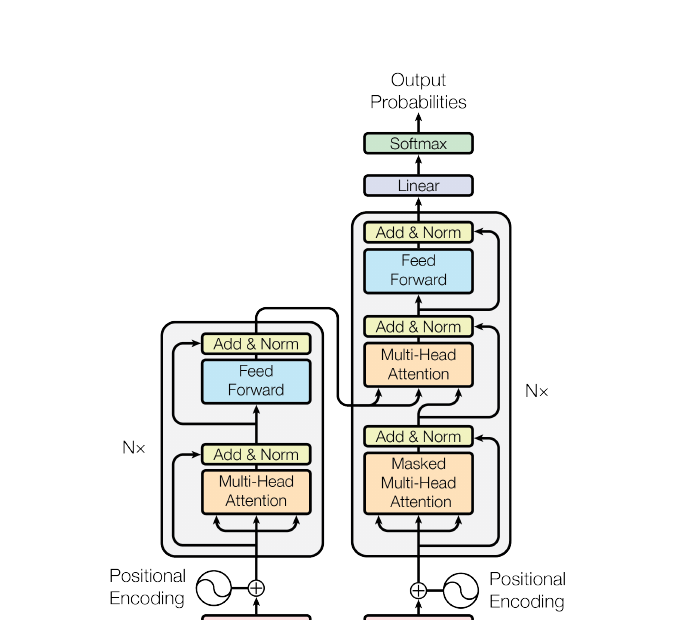
\includegraphics[width=0.64\textwidth]{figures/chapter2/refs/fig_transformer_ref.png}
    \caption{Transformer基本结构参考图，引自文献\cite{52vaswani2017attention}}
    \label{fig:ch2_transformer_ref}
\end{figure}

\subsection{大语言模型领域适配与知识增强原理}
\ensubsection{Principles of Domain Adaptation and Knowledge Enhancement for Large Language Models}

当大语言模型用于专业领域分析任务时，模型输出通常需要同时满足术语约束、结构约束和依据约束。若缺少这些约束，模型虽然能够生成表面连贯的回答，但结果未必稳定可靠\cite{Choi2024,Jiang2025}。

在不改变模型参数的前提下，知识增强通常通过输入侧注入任务约束、示例信息和外部知识来实现。设原始问题为 $x$，任务指令与格式约束为 $p$，示例集合为 $E$，外部知识上下文为 $K$，则增强后的模型输出可抽象表示为
\begin{equation}
    y=\mathcal{M}_{\theta}(x,p,E,K)
\end{equation}
其中，$\mathcal{M}_{\theta}$ 表示参数固定的大语言模型，$p$ 用于约束回答任务和输出形式，$E$ 用于提供少样本示例，$K$ 用于补充术语解释、条件范围和结论依据。该式表明，知识增强的核心是在模型输入中显式加入任务所需的结构约束和外部知识。

在这一机制下，提示词约束、少样本示例和结构化输出要求主要用于控制模型的输入输出形式\cite{Polak2024}。当任务涉及术语解释、条件比对和结论依据说明时，还需要接入外部知识，以补充模型参数中难以显式更新和直接追溯的内容\cite{Mostafa2024}。因此，大语言模型更适合承担知识增强链路中的语言处理与生成任务。

在专业领域应用中，常见的模型适配路径主要包括领域微调和检索增强。前者主要通过在特定任务或领域语料上继续训练提升模型适应性，后者主要通过外部知识检索补充推理依据\cite{Soudani2024,lewis2020rag,Mostafa2024}。对于知识更新频繁、条件约束较多且需要证据支撑的科研分析任务，检索增强通常更适合与后续的结构化知识表示和检索链路配合使用。

\subsection{图结构知识组织基本原理}
\ensubsection{Basic Principles of Graph-based Knowledge Organization}

在科研分析任务中，知识对象往往不仅是孤立文本片段，还包括对象、条件、结果和机理概念之间的对应关系。若仅以文本段落或向量表示保存相关信息，虽然可以保留局部语义，但对象之间的关系结构、条件范围和来源依据较难显式表达。为此，通常需要进一步引入结构化知识表示，对多源信息进行统一组织\cite{Statt2023,Venugopal2024}。

图结构知识表示能够较好地组织对象、条件、结果和解释之间的关系。其基本思想是将知识表示为由节点和边组成的网络结构，其中节点用于表示对象单元，边用于描述对象之间的关联关系。其一般形式可写为
\begin{equation}
    \mathcal{G}=(\mathcal{V},\mathcal{E},\mathcal{A})
\end{equation}
其中，$\mathcal{V}$ 表示节点集合，$\mathcal{E}$ 表示边集合，$\mathcal{A}$ 表示与节点或边相关的属性信息。节点可用于表示文献、样品、工艺参数、形貌指标或机理概念等对象，边用于表示对象之间的对应、作用或来源关系，属性则用于保留条件范围、单位、时间信息和证据标识等内容。

在局部关系层面，图结构中的单条知识关系还可抽象写为
\begin{equation}
    \tau_{ij}=\bigl(v_i,r_{ij},v_j,a_{ij}\bigr)
\end{equation}
其中，$v_i$ 和 $v_j$ 分别表示起点节点和终点节点，$r_{ij}$ 表示关系类型，$a_{ij}$ 表示与该关系相关的属性集合。$a_{ij}$ 通常包含条件范围、来源标识、时间信息和证据编号等内容。采用这种表示方式后，知识对象之间的关系不仅能够被显式保存，还能进一步保留关系成立的适用条件和来源依据。

相较于纯文本块或单一向量表示，图结构不仅保留内容本身，还能够显式表示对象关系、条件范围、证据来源和上下位关联，因此更适合承担知识组织与结构保存任务。这一组织思想与科研数据可追溯、可复用的基本要求是一致的\cite{Wilkinson2016FAIR,Lebo2013PROVO}。图~\ref{fig:ch2_kg_ref} 给出了知识图谱原始参考图，其节点、关系和属性的表达方式可为后续中文化改绘提供参照\cite{Hogan2021KG}。

\begin{figure}[htbp]
    \centering
    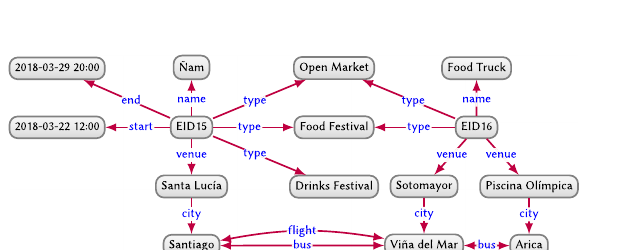
\includegraphics[width=0.78\textwidth]{figures/chapter2/refs/fig_kg_ref_hogan.png}
    \caption{知识图谱基本结构参考图，引自文献\cite{Hogan2021KG}}
    \label{fig:ch2_kg_ref}
\end{figure}

\subsection{检索增强与证据组织基本原理}
\ensubsection{Basic Principles of Retrieval Augmentation and Evidence Organization}

检索增强的基本思想，是在生成之前先从外部知识源中检索相关信息，再将检索结果与用户问题一并输入模型，从而提高回答的针对性和可信度\cite{lewis2020rag}。在科研分析任务中，检索返回的结果不仅需要相关，还需要能够支撑后续对象判定、条件比对和结果说明。图~\ref{fig:ch2_rag_ref} 给出了 Lewis 等\cite{lewis2020rag} 在原始论文中提出的 RAG 结构参考图，其展示了查询编码器、检索器、文档索引和生成器之间的连接关系。

\begin{figure}[htbp]
    \centering
    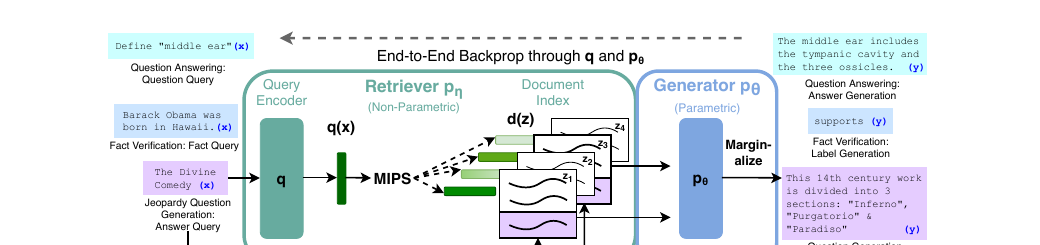
\includegraphics[width=\textwidth]{figures/chapter2/refs/fig_rag_ref.png}
    \caption{RAG基本结构参考图，引自文献\cite{lewis2020rag}}
    \label{fig:ch2_rag_ref}
\end{figure}

在科研文本检索任务中，候选条目通常需要先转化为可以计算相似度的表示形式。传统稀疏检索主要依托倒排索引和词项权重完成候选召回，较有利于保持专业术语、参数符号和条件短语的精确匹配，但对语义近邻和跨表述变体的覆盖相对有限\cite{Mostafa2024}。以 BM25 为代表的稀疏检索评分形式通常可写为\cite{Robertson2009BM25}
\begin{equation}
    S_{\mathrm{sparse}}(q,d)=\sum_{t\in q}\mathrm{IDF}(t)\cdot
    \frac{f(t,d)(k_1+1)}{f(t,d)+k_1\left(1-b+b\frac{|d|}{\mathrm{avgdl}}\right)}
\end{equation}
其中，$f(t,d)$ 表示词项 $t$ 在候选条目 $d$ 中的出现频次，$|d|$ 表示条目长度，$\mathrm{avgdl}$ 表示候选集合中的平均长度，$k_1$ 和 $b$ 为控制词频饱和和长度归一化的参数。该式说明稀疏检索主要依赖词项匹配程度和文档统计特征完成候选排序。稠密检索则通过编码模型将查询和候选条目映射为向量表示，再利用向量空间中的距离或相似度衡量二者的语义接近程度。句向量模型和双编码器结构是较常见的技术形式，其优点在于能够将不同表述但语义相近的内容映射到相邻空间位置\cite{Reimers2019SentenceBERT}。

对查询 $q$ 和候选条目 $d$ 而言，稠密表示的一般形式可写为
\begin{equation}
    \mathbf{z}_q=f(q),\qquad \mathbf{z}_d=f(d)
\end{equation}
其中，$f(\cdot)$ 表示向量编码函数，$\mathbf{z}_q$ 和 $\mathbf{z}_d$ 分别表示查询与候选条目的向量表示。对应的语义相似度通常可写为
\begin{equation}
    S_{\mathrm{dense}}(q,d)=\cos(\mathbf{z}_q,\mathbf{z}_d)=\frac{\mathbf{z}_q^{\top}\mathbf{z}_d}{\lVert \mathbf{z}_q\rVert \lVert \mathbf{z}_d\rVert}
\end{equation}
该式反映了稠密检索通过向量方向相近程度衡量语义相似性的基本思想。

在科研任务中，研究者关心的往往不是单一事实，而是条件、现象和解释之间的关联过程。仅依赖关键词检索容易忽略语义近邻，仅依赖向量检索又可能弱化条件约束和专业术语的精确匹配，因此混合检索逐渐成为更常见的技术路线\cite{Mostafa2024}。在混合检索阶段，稀疏检索结果与稠密检索结果通常采用加权融合方式共同参与排序，其一般形式可写为
\begin{equation}
    S_{\mathrm{hyb}}(q,d)=\alpha S_{\mathrm{sparse}}(q,d)+(1-\alpha)S_{\mathrm{dense}}(q,d)
\end{equation}
其中，$S_{\mathrm{sparse}}$ 和 $S_{\mathrm{dense}}$ 分别对应关键词匹配得分与语义相似度得分，$\alpha$ 用于控制两类信息在候选排序中的相对权重。该式表明，混合检索的核心在于同时保留术语精确匹配能力和语义召回能力。

证据组织关注的是如何将检索结果按对象、条件、来源和关系进行重新整理，使输出内容能够直接支撑后续分析判断。单条证据可进一步抽象表示为
\begin{equation}
    e_i=(o_i,c_i,r_i,\pi_i)
\end{equation}
其中，$o_i$ 表示证据对应的对象单元，$c_i$ 表示适用条件，$r_i$ 表示核心关系或判断，$\pi_i$ 表示来源与定位信息。证据不仅要相关，还应能够回溯其来源、生成过程和适用条件\cite{Soudani2024}。因此，检索增强通常还需要与前述图结构知识表示配合使用，才能将返回结果整理为可分析、可追溯和可复用的知识依据。

\section{小结}
\ensection{Summary}

本章围绕后续章节所需的两类基础展开，即碳纳米管阵列制备工艺基础和知识增强方法基础。前一部分说明了碳纳米管阵列常见制备路线、CVD 生长过程以及关键工艺参数与形貌之间的联系，为后续工艺变量分析提供过程背景。后一部分介绍了 Transformer 与大语言模型原理、大语言模型领域适配与知识增强原理、图结构知识组织原理以及检索增强与证据组织原理，为第三章的多源知识建模与证据链检索方法提供支撑。通过这些准备，后续章节中的知识增强分析和工艺—形貌关系研究能够更自然地衔接起来。
